% Created 2020-10-29 Thu 17:07
% Intended LaTeX compiler: pdflatex
\documentclass[12pt,titlepage]{article}
\usepackage[utf8]{inputenc}
\usepackage[T1]{fontenc}
\usepackage{graphicx}
\usepackage{grffile}
\usepackage{longtable}
\usepackage{wrapfig}
\usepackage{rotating}
\usepackage[normalem]{ulem}
\usepackage{amsmath}
\usepackage{textcomp}
\usepackage{amssymb}
\usepackage{capt-of}
\usepackage{hyperref}
\usepackage[natbib=true]{biblatex} \DeclareFieldFormat{apacase}{#1} \addbibresource{./refs.bib}
\usepackage{parskip}
\usepackage{listings} \usepackage{color} \definecolor{dkgreen}{rgb}{0,0.6,0} \definecolor{gray}{rgb}{0.5,0.5,0.5} \definecolor{mauve}{rgb}{0.58,0,0.82} \lstset{frame=tb, language=Java, aboveskip=3mm, belowskip=3mm, showstringspaces=false, columns=flexible, basicstyle={\small\ttfamily}, numbers=none, numberstyle=\tiny\color{gray}, keywordstyle=\color{blue}, commentstyle=\color{dkgreen}, stringstyle=\color{mauve}, breaklines=true, breakatwhitespace=true, tabsize=3}
\usepackage[T1]{fontenc}
\usepackage{setspace}
\usepackage[english]{babel}
\usepackage[hyperref,x11names]{xcolor}
\usepackage[colorlinks=true,linkcolor=SteelBlue4,urlcolor=Firebrick4]{hyperref}
\author{Nandaja Varma Nandakumar}
\date{}
\title{Stateful FaaS}
\hypersetup{
 pdfauthor={Nandaja Varma Nandakumar},
 pdftitle={Stateful FaaS},
 pdfkeywords={},
 pdfsubject={},
 pdfcreator={Emacs 27.1 (Org mode 9.3.7)}, 
 pdflang={English}}
\begin{document}

\maketitle
\begin{abstract}
Serverless Computing is an up and coming platform as a service offering 
where the cloud provider manages and allocates
resources needed to keep the application running. This lets the developer focus on the application development
and not on server maintenance. Alongside off loading the provisioning and
maintenance of the server, Serverless computing also reduces resource waste
by scaling up and down the allocation depending on the load and the
configurations. The users only pay for the resources that were used by the
application thereby saving huge operational cost on their infrastructure
hosting.

Although Serverless might sounds like the holy grail of application hosting, the 
current state of art technology fall short in several places to meet the industrial
requirements. Data intensive applications, streaming applications, and
distributed computing are some of the fields that could be benefited heavily by
implementation on Serverless platforms in terms of ease of development,
efficiency and cost. But all the existing platforms offer very
poor performance in these fields and works mostly via workarounds and n number
of third party tools.

This thesis analyses the Serverless paradigm in depth,
pointing out the reasons for this reduced adaptability. To solve these issues, we propose a lightweight
extension to an existing Open Source Serverless platform, OpenFaaS, by provide
flexibility, scalability and adaptability, while making sure not to violate the notion
of functions. Our implementation tries to reduce the operational gap between the
industrial applications and theoretical ideas produced by researches in the
academia in the past few years.
This thesis also offers a deep study of the full potential and limitations of
Serverless thereby making it clear to the reader why more innovations are
necessary in this field.

\end{abstract}

\setcounter{tocdepth}{4}
\tableofcontents


\section{Introduction}
\label{sec:org83bb847}

Serverless can easily be considered as the new generation of platform as a
service. It can be thought of as an infrastructure where the programmer send
their application as functions in a predefined format, in a supported
programming language as documented by the provider. This function get hosted at
a certain endpoint which can be triggered with certain events supported by the
platform. In short, instead of having continuously running servers, functions operate as
event handlers and when the functions execute, the equivalent CPU usage is paid
for by the user. This has huge economical and architectural implications that is
still waiting to be explored in its full power. While the developers worry about
the logic of handling the requests/events, the infrastructure provider takes
care of receiving the request, responding to them, capacity planning, task
scheduling, and operational monitoring\cite{gotoconf}.

In the current industrial applications, data intensiveness of the applications are increasing
day by day paving way to adopt several resource heavy tools to do stream
processing, distributed processing etc. More than often CPU and memory loads in
these machines tent to vary a lot and rather than having a dedicated server to accommodate the whole range
of requirements, it makes perfect sense to convert it into a Serverless workload
thereby saving up on operational cost, resource waste, and ease of development.
Having said that, the current commercial offerings of Serverless do not work
very great with such workloads.

This is mostly due to the sheer
nature of the Serverless paradigm of being completely stateless, thereby forcing
the developers to use external block storages for data store and communication.
In this thesis, we try to extend Serverless to leverage its full potential by
introducing an efficient form of state thereby providing flexibility, scalability and
adaptibility at the same time not violating the notion of functions in these platforms.
We will be extending an Open Source serverless platform called OpenFaaS
considering its simplistic and expandable architecture.

Currently most of the commercial serverless offerings are closed source
and vendor locked in to their respective platforms by cloud providers. But in the
past couple of years the field has gotten a lot of traction in the academia and
a lot of Open Source alternatives are being widely adopted. This being the case, a lot
of these works hasn't been properly applied in the industry, some because of
the absense of proper integrations with the industry standard tools, and some
because of the operational gap between the theoretical ideas and the
practicality or usability in the field. This thesis tries to reduce that
gap by proposing a very secure and multi-tenant implementation of a
state-ful Serverless setup which can be easily used for production quality
applications. A focus on the possibility to monitor the application performance
and usage provides a possibility to do fine grained billing of the resources and thereby
contributing to the easy adaptability of our extension.

Using our proposed Serverless setup, we try to efficiently run a
Extract-Transfer-Load(ETL) workload on streaming data. ETL basically is a pipeline that involves receiving data
from source, cleaning and transforming it, and loading it to a sink. We will
split the whole operation into multiple functions as per the Serverless notion
and have them communicate data and state internally to complete the pipeline
thereby reducing the latency and external bottlenecks.

This document describes more on Serverless paradigm, the shortcomings of it, the
ones we are trying to solve, our solution and evaluation. It is split into
several sections as follows:

In Section 2, we go a bit in depth to understand the history of cloud
infrastructure and the technological innovations that led to Serverless
paradigm. We also look in detail at the characteristics and nature of
Serverless. We look at some commercial Serverless offerings and understand how
in the programming world Serverless has influenced even in the way of developing.
We will also see what limitations it holds at its current state of evolution and
on solving which issue are we particularly interested in, in the scope of this
thesis.

In Section 4, we look at the current state of research in the field of
Serverless technologies and some related works.

In Section 3, We present the proposed solution for our Serverless setup going
into detail about how certain unacceptable limitations can be overcome.

In Section 4, the implementation of the system including the architecture and
the tools used is presented.

In Section 5, we go on with the evaluation of our system as opposed to standard
Serverless workloads.

We move on to Section 6 to understand the limitations of our proposed system.

In Section 7, the future work that can be done in this direction is laid out
before the reader.

\section{Background and Motivation}
\label{sec:orgd0ddcb3}
The term serverless have been vaguely thrown around the domain of cloud
infrastructure in the past decade as the breakthrough resource(and hence money)
saving tool that lets the developers focus on application logic rather than the
deployment and server maintenance. Having said that, it is often hard to define
what exactly serverless is since the service offering tend to change based on
the cloud provider and the interpretations of the users. It is fair to say that
serverless is a huge leap in the direction of using computational power as a
resource which can be paid for as per the usage.
Although the terminology is irrelevant, we will be focusing on the serverless
offering called Function-as-a-Service(FaaS) where the cloud providers offer a
platform to which we can upload our application code to(complying to the API
rules) and get uninterrupted service of the same at an endpoint irrespective of
the traffic or data load. Paying only for what resources has been used adds to
the attraction of the domain.
In this section, we will understand more about this technology, the
popular commercial offerings the same, and its limitations and the current state
of research. 
We will also analyze the popular data processing and streaming pipelines in the
industries these days and why serverless computing fall short in being the right
tool of development and deployment here.
\subsection{Evolution of cloud resource management}
\label{sec:org6cf6a24}
In the past 3 decades, software deployments and infrastructure management has
seen a lot of innovation and evolution. Before diving into the current
industrial standards, it is important to understand the evolutions in this field
to get a better grasp on the technological innovations that bought this about.


\subsubsection{Dedicated servers}
\label{sec:org225c375}
Even as recent as 15 years ago this was the industry standard for deployments. Dedicated servers
are physical machines. The general practice was to have server racks on the premise
of the company which are maintained by system administrators and all your
software is
hosted there. Although this method offers advanced security and high
availability, it is often common that a lot of physical resources were
underutilized and each resource was for single client. Not to mention the
environmental impact of the reserved heavy hardware which leaves a heavy carbon
footprint and e-wastes.


\subsubsection{Dedicated virtual machines(BaaS)}
\label{sec:org014b3de}
Virtualization technology changed the face of software infrastructure by decoupling
applications from the underlying hardware. Virtualized servers are not physical
machines, they are a software construct. Virtual servers run on dedicated
servers, the resources of which are divided between several virtual servers.
To get slightly technical, virtualization usually involves installing a virtualization software(Hypervisor) on an
existing operating system and then having multiple operating systems on it,
sharing all the resources of the underlying operating system, yet providing
great security and isolation.

\begin{figure}[!h]
    \caption{Figure 1: Virtualization through hupervisors}
    \centering
    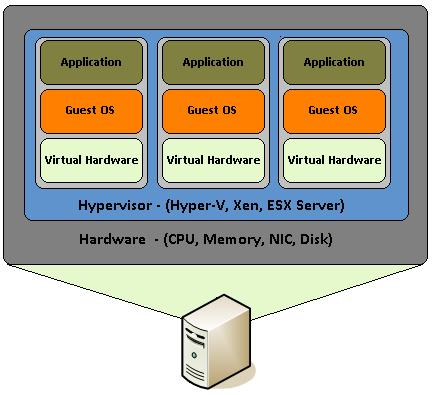
\includegraphics[width=80mm]{./thesis_images/virtual_machines.JPG}
    \label{fig:testing the label}
\end{figure}


Although applications in hosted on the virtual machine suffers from a heavy
input/output and network overload because of the added layer of indirection,
this technology reduces the resource waste to a great extend. The enterprises could share their hardware into
multiple virtual machines and have different hosting and computation in each of
the them. System administrators started splitting up their bare metal resources
among multiple Virtual Private Servers(VPS) by the help of virtualization
software. Each VPS would give you the feeling
of having a real system although it is a virtualized system which is sharing the
resources with other VPSs. This reduced a lot the amount of work and energy spent on
maintaining server racks along with the terrible underutilization of resources.

More and more companies started adapting this technology and in early 2006
Amazon Web Services(AWS) re-launched themselves as a platform that offers
computing and storage space to developers and enterprises on an on-demand basis
revolutionizing how companies were designing their system architecture. Soon
after Google and Microsoft followed suit with their cloud infrastructure
platforms offering similar services. All these providers function by maintaining
huge, dedicated server farms across the globe to provide the necessary resources
to the customers.

These kind of services, generally called as Infrastructure as a Service(IaaS) or
Platform as a Service(PaaS), went through a
series of changes during the past decade. On-demand compute instances to
completely managed deployment services(eg: Google App Engine), Pay per use block
storages(AWS S3) to fully managed dedicated relational databases(Google Cloud
SQL, AWS RDS, etc.) a lot of really efficient and interesting services started
to be available for the developers disposition. The billing scheme of these
services also started to be quite flexible even allowing a per second billing
plan in the past couple of years by Google.

It is also worth noting that with the advent of virtualization, the job profiles
in several companies shifted from having a system administrator role to 
having profiles called DevOps(development and
operations) who are application developers focusing on the provisioning of the
virtual machines to deploy their applications. Although IaaS solved a lot of
hassle around infrastructure provisioning, the systems and load of the
applications still remained independent. Applications always had dedicated virtual machines
even if the load/traffic to and fro the application is not constant. This meant that a
lot of resources were still being wasted.

\paragraph{Linux Containers}
\label{sec:org0911da7}
A game changer in the world of virtualization was containerization. Containers
are yet another packaged computing environment that combine various IT
components and isolate them from the rest of the system just like a virtual
machine would. It was developed to solve a lot of problems with virtual
machines. The purpose of the containers is to encapsulate an application and its
dependencies within its own environment. This allows them to run in isolation
while they are using the same system resources and the same operating system.
Since the resources are not wasted on running separate operating systems tasks,
containerization allows for a much quicker, lightweight deployment of
applications. Each container image could be only a few megabytes in size, making
it easier to share, migrate, and move. Figure 2 shows the difference in the
isolation levels of containers and virtual machines.
[containers]CITE Even though Linux Containers
have existed for a very long time, in the past decade, containers were made a
lot more approachable and adaptable as a
technology by the advent of communities like Docker and rkt.

\begin{figure}[!h]
    \caption{Figure 2: Virtual Machines Vs Containers}
    \centering
    \includegraphics[width=80mm]{./thesis_images/VM_image.PNG}
    \label{fig:vm_vs_containers}
\end{figure}

The light weight of the containers
made it the ideal candidate for running applications. What makes container based deployments special
as opposed to the ones deployed directly on the host is the consistency of the environment. The application
execution environment can be recreated and ported from one system to another without affecting the functionality
of the application or having to reinstall the whole binary dependencies on the new machine. Reproducability of the
production environment even in the local exactly, meant that the development/testing cycle became much more efficient.
The isolated package of the application, enveloped as a container image, is
agnostic of the operating system it runs on opening new possibilities for the
deployment. One could also limit and fine tune the resources used by a running
containers giving a lot more control over the application.

\paragraph{Autoscaling}
\label{sec:org8d376a7}
The ease in which one can limit the resources and tweak the runtime parameters externally contributed heavily
to the service offering called autoscaling which basically meant resources for an
application runtime were added or removed as per the usage. All the commercial
cloud providers started offering the aforementioned service in different
flavors. Autoscaling on EC2 or Google Compute, AWS Fargate, etc. are some examples.

In the past two years, innovations have taken a leap in the field of isolation
environments, introducing solutions like AWS Firecracker, Cloudflare workers,
etc. to the community. These solutions aim at mitigating the shortcomings of
Containers which we will discuss in Section 2.2.4

\subsubsection{Serverless}
\label{sec:org3b953a9}
Like mentioned earlier, in the past two years the terms Serverless and Function-as-a-Service are quite
often used interchangeably. In terms of the resource reservation, Serverless can
be considered as a platform as a service solution that scales. Your application
will always have enough and only enough resources dedicated to it. It will scale
up and down based on the load and traffic and the developer only pays for the usage.
This paradigm of autoscaling has been hence applied even to database storage
solutions by major cloud providers such that even the block storage is allocated
based on usage and there will be a burst of reservation as soon as a certain
limit is reached.
The pioneers of this technology can be considered as the proprietary service
Lambda by Amazon Web Services[CITE]. Several other cloud providers followed suit
with similar platforms specific to their infrastructure.
The nature of serverless makes it attractive for both developers and the cloud
providers since in the case of former, it means paying much less and in case of
the latter, it means they can easily provide shared tenant resource allocation
units.

We will dive more into the properties and nature of the solution
Function-as-a-Service(FaaS) in the following session. 

\subsection{FaaS}
\label{sec:org95ea4f5}
So far, we have covered the infrastructure management style of FaaS or
Serverless in general. Let us get a bit in detail into the specifics of the
hosting platform that provides the FaaS functionality.

Most FaaS platforms being closed source, provides the client API for developers
to supply a package including their code and dependencies to. Most platforms
supports a limited set of programming language runtime although it is usually
possible to do workarounds to deploy custom runtime. Behind the screen,
the platform containerizes the application and deploy it so as to get triggered
via pre-defined hooks specified by the developer. The infrastructure also provides endpoints or
interfaces to specify the maximum and minimum CPU and memory allocated for the
application, the maximum timeout for the application(although there is a
hard bound on this imposed by the infrastructure provider usually). To
understand the flow of FaaS workloads, it is important to be aware of the
following properties of the platform.

\subsubsection{Properties of FaaS}
\label{sec:org3032d42}
\paragraph{Statelessness}
\label{sec:org45db990}
Statelessness in deployments is a conscious decision that was taken during the
conception of the Serverless infrastructure model to make the management of the
platform straight forward and less cumbersome. Statelessness simply means that
the applications that are to be deployed on the said platform exists as
independent functions that are pure in nature. As in, the same data input given
to the function always produces the same output at any point in time. This can
be considered as the side-effect less programming. The data source and sink of
the function can be any supported platform or tool as per the requirement, but
there won't be any intermediate state or cache for the function. This means that
the function at any execution will have no information about the previous
execution unless explicitly specified.

The main advantage with this method for the infrastructure manager is pretty
obvious. The fact that there are no volumes necessary to store any internal
state means that the function can be scaled up and down independently and the
whole infrastructure can stay elastic. Along with this, the provider can
schedule the function in any node in the cluster that they use to host the
application, move it around as per the usage burst, have multi-tenant
deployments in a single machine ensuring the proper isolation for maximum
profitability, and the list goes on.

In short, the notion of function is of prime importance in a
Function-as-a-Service workload like the name suggests.

\paragraph{Triggers}
\label{sec:org3459818}
The functions that are hosted on a FaaS solution need to get triggered on a timely
basis or based on an event. Usually most cloud providers provide more than a few
ways to trigger the functions which the developer can choose from. Some of the
most common triggers for FaaS applications are
\begin{itemize}
\item HTTP requests: An endpoint will be provided by the platform for the function that was deployed.
\end{itemize}
This endpoint can be called as an REST API endpoint and the event handler of
the function will get the payload from the call.
\begin{itemize}
\item Data arrival in a storage or data broker system: This is the most popular and heavily used triggering mechanism in FaaS. The idea
\end{itemize}
is that the function gets triggered as soon as a new data arrives in whatever
format at a particular storage setup. This can be arrival of a file object in
the S3 block storage, arrival of streamed data in Kafka message broker system,
etc. This method is the most suited for big data and streaming data applications
since the function can be activated as soon as the new data is detected in the
source. Usually the FaaS infrastructure provide supports more than a bunch of
source storage to be used as the sources for the trigger.
\begin{itemize}
\item Cron: Another very common way to trigger function is based on a schedule. The
\end{itemize}
programmer can choose how often the function should be triggered on what days of
the week, month, year, etc. 
\paragraph{Parallelism}
\label{sec:org6b2cfeb}
\paragraph{Billing}
\label{sec:org2972d4d}
\subsubsection{How programming models are getting affected by this}
\label{sec:orgd3763b6}
\paragraph{Faas + Microservices}
\label{sec:org545c527}
In Software Systems Design, a very heavily discussed topic is if to design the
application in a monolithic fashion or a micro-services fashion. Monolith is the
kind of design pattern where you have one big application doing multiple
functions and maintained as one solid stack. On the contrary, when one designs
their app in a microservices pattern, they will have split up their application
into multiple smaller parts which can be independently built and deployed, and
yet working together with inter app communications. Both of these methods has
its advantages and challenges. When monoliths are easier to develop and
maintain, it can be very hard to test and manage due to the size, and usually if
one part is buggy, it tends to break the whole system. On the other hand,
microservices, since they work as independent units don't usually affect each
others working and can be very easily tested and maintained. It is although
often a very tedious task developing a system that fragmented and maintaining it
that way. 

With the advent of FaaS, a very interesting pattern has been adapted in the
industry. The pattern pushed microservices one step further. The idea is that
instead of having microservices that are available and on at all time, the huge
applications are split up into functions that can be deployed to a FaaS
infrastructure and triggered with the help of HTTP endpoints to act as a part of
web application setup. This method is very effective resource usage wise and
much easier to deploy and manage compared to vanilla microservices which has to
be built and deployed independently.
\paragraph{Statelessness a.k.a Functional programming model}
\label{sec:orga99b187}
Like mentioned earlier, the notion of function is very important for the
serverless platforms. It is intrinsically linked with functional programming. It
is very interesting to note that Amazon named their FaaS solution Lambda which
is a very basic concept of functional programming. Stateless clean functions
that produce no side effect was objectively the perfect choice for an
infrastructure solution of this scale.

What this change bought about is a thriving interest in functional programming
languages. A lot of the functional programming languages belonging to the LISP
family and some purely functional ones have seen a very increasing adaptation in
the past few years in Serverless platforms. Since these languages are perfectly
suited for stateless program it is only natural that they can be efficiently
used to code for this environment.
\subsubsection{Popular commercial offerings}
\label{sec:org4c745ef}
\paragraph{AWS Lambda}
\label{sec:orgc701811}
\paragraph{Google cloud functions}
\label{sec:org5c4c8ca}
\paragraph{Azure functions}
\label{sec:orgd572f27}
\subsubsection{Where Serverless computing fall short}
\label{sec:org1fb5283}
Although serverless computing might sound like the silver bullet of the
deployment solutions, it is a field that is still being rapidly grown and
researched on. There are several staggering shortcomings for this technology
that makes it unsuitable for certain applications. The current offering have the
following noticeable limitations.
\paragraph{Lack of state}
\label{sec:org97f89a5}
As mentioned earlier, statelessness is a primary nature for serverless workloads
making it easy to deploy and port agnostic of the environment and server.
Hence serverless/auto-scaling paradigm generally push for a development style
involving no state to make the infrastructure simple, encouraging a functional
style of development. Although this can contribute to easily scalable and
parallelisable applications, it often limits the technology from being adapted
in applications that are data intensive and/or requires faster response times.
The fact that serverless functions don't store any intermediate state requires
the application developers to use a block storage to store the data and state
after the execution. This basically means communication via slow storage and
adds a lot to the latency. This discourages the use of serverless in distributed
computing which is actually a domain that needs very fine grained communication
between the functions and usually a lot of resources are wastefully dedicated to
ensure high availability.

A function during execution has no clue of the previous executions and its
results. Which is something that is usually very basic for data analysis
operations. The developers in this case are forced to send the data after each
execution to a block store and retrieve the data from the block store before the
next execution. Other than the input output overhead and the network latency
this adds, it is a violation of the elastic nature of the Serverless
paradigm.

\subparagraph{I/O Latency}
\label{sec:org79ad623}
Like was mentioned earlier, FaaS have had a lot of influences in the system
architecture and programming paradigms like would with any new infrastructure
management system. It is quite unfortunate though that, even with a paradigm
with such huge potential, FaaS is very conventional when it comes to its data
engineering architecture. Functions are run in isolated units separate from the
data or data store. This is actually a very huge system design anti-pattern
because Input/Output have and will remain to be a bottle neck even with heavy
memory and huge number of dedicated cores to a function. The pattern where the
data is taken to code as opposed to code to data adds to the latency, cost, and
inconvenience. For the clarity of the reader, an example of a code shipping
architecture is procedures that you run in databases. The code is moved to the
data than the other way around in this.

\paragraph{Coordination issues among functions}
\label{sec:org336996d}
As we saw in the previous sections, FaaS workloads are usually containerized by
the cloud provider to deploy it easily in their node pool or cluster. By nature,
docker containers are indiscoverable units that need to be opened up explicitly
to the network of the host machine. Meaning that, we cannot explicitly address
the docker container directly using an IP address or an endpoint. Cloud
providers do not open up the container to the network consider the potential
security issues this can cause and the necessity of state in this case. They
provide handles to communicate with the function or trigger-able entry points,
but no direct network addressability.

What this implies is that, if the developer has multiple functions that has to
be composed together to form a pipeline, rather than triggering each other
internally and directly, the developer will have to hack around by either
triggering it via an HTTP endpoint if the provider allows that, or like was
mentioned in the previous point via an external block storage, or other external
queueing systems they provide, etc. In either of these
scenarios, it is hard to avoid added latencies. 

This makes FaaS particularly inefficient for applications like distributed
computing when it depends on very fine grained communication between the
functions. With FaaS we can only ensure very weak consistency across function
storages making it a pretty bad candidate. What this also means is that there is
no way we can actually have efficient parallelism even if we have many powerful
cores installed over the current state of FaaS since the block storage will
always be a bottleneck.

It goes without saying that most big data applications that need ephermeral
storages between function executions suffers from the very similar kind of
latencies as well. This includes function compositions like ETL on streaming and
batch data alike.

CITE[onestepforward]

\paragraph{Vendor lock-in}
\label{sec:org1f715ab}
It is no secret that the most widely used FaaS/serverless offerings are the ones by
proprietary cloud providers where they hand twist the developers into complying
to their programming environment and runtime thereby forcing devs to use their
technologies. What such practices contribute to is limited innovations and
development around the paradigm of Function as a service itself and people
re-inventing the wheel by creating custom made code and hack to fit each of
these provider runtime.

In a system like FaaS, where you are basically out-sourcing the whole setup of
your application to a vendor, the fact that the whole ecosystem is closed source
and uses the tools developed by the vendor only means that the user has near to
zero control over the infrastructure and the pipeline is not transparent at all
for any kind of performance optimization or fine tuning.

\paragraph{Fixed timeouts}
\label{sec:org398b0f7}
This is the one of the other bigger reasons that hinder the usage of FaaS in big
data applications. In applications that involve heavy number crunching
algorithms, there are chances that often the function needs to run for a longer
period of time. Current commercial FaaS offerings has a fixed timeout, exceeding
which the function execution is automatically terminated irrespective of the
stage of the execution. The fact that the platform offer little to no control
over this discourages the developers to use the tool.

Currently the maximum timeout for function execution in AWS and GCP platforms
for the FaaS setups are 15 minutes and for Azure functions it is 10 minutes.
These are all extremely bounding as conditions especially for functions that are
composed and a function should wait for the other functions to finish executing. 

\paragraph{Cold Start}
\label{sec:orgf184eb3}
Cold start it the delay that the function incurs after the invocation or
triggering of the function till the execution of the function. In the
background, FaaS uses containers to encapsulate and execute the functions. When
an user invokes a function, FaaS keeps the container running for a certain time
period after the execution of the function (warm) and if another request comes
in before the shutdown, the request is served instantaneously. Cold start is
about the time it takes to bring up a new container instance when there are no
warm containers available for the request CITE\{\href{https://medium.com/faun/on-the-serverless-cold-start-problem-2fc0797da5cc}{Blog}\}. In most platforms
serverless latency on average is measure to as 1-3 second CITE\{\href{https://mikhail.io/2018/08/serverless-cold-start-war/}{BLOG}\}, which can
have very dramatic impacts when it comes to certain workloads. According a 2018 survey, this is the third biggest concern developers have
regarding the serverless platform CITE\{\href{https://www.serverless.com/blog/2018-serverless-community-survey-huge-growth-usage}{BLog}\}. 

The cold start time in-fact is overblown by several factors in the
infrastructure. All the popular commercial FaaS offerings suffer from a cold
start time. It can referred that irrespective of the language runtime used, the
start time tend to be almost the same on a platform. The main deciding factor is
the dependencies that were packaged for the application which obviously makes
the container slower to start because of the heaviness. Figure 3 shows the cold
start time differences across different commercial cloud providers under
different runtime and different dependencies.

\begin{figure}[!h]
    \caption{Figure 3: Cold start across cloud providers [[https://mikhail.io/2018/08/serverless-cold-start-war/][CITE]]}
    \centering
    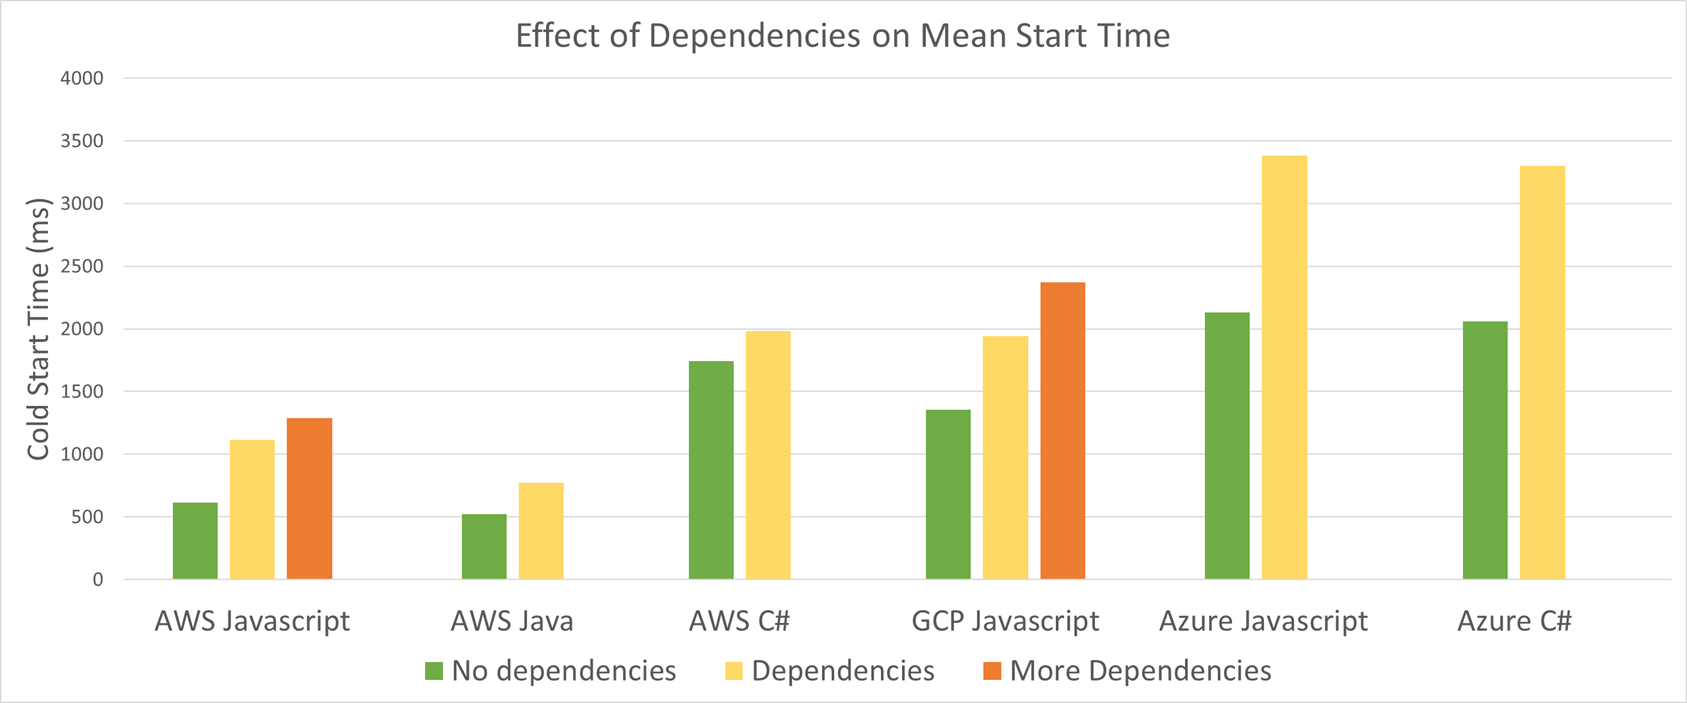
\includegraphics[width=80mm]{./thesis_images/cold_start.png}
    \label{fig:cold_strt}
\end{figure}

A solution for this problem, other than keeping the dependencies small, is to
have a warm function up at all times so it can handle the request right away for
time sensitive applications. The problem here though is that most commercial
offerings do not offer this option. Instead the developers are forced to keep
pinging the function to keep it warm for the next trigger. This is a very hacky
solution and reduces the whole efficiency of the platform in general. Most of
the cloud providers are although aware of this problem and are trying to be
innovative and introduce lighter alternatives to Linux containers in the FaaS
platform these days.

\paragraph{Security issues in a multi-tenant environment}
\label{sec:org401bf28}
Like was previously mentioned, the whole FaaS infrastructure offering is
economical for the cloud provider because they get to share their node pool
among all their standard customers making the resource cost for them very low.
The problem with this practice though is that this introduces safety issues for
the data that is executed in the machines. Linux containers are not
particularly secure as an isolation mechanism since they share a Kernel with the
host operating system. This means that any bug or back door introduced to the
Kernel get affected to all the containers as well exposing the customer data at
a very high risk. This is an issue that is actively being worked on by
companies. Till a while ago, the solution for this was to encapsulate the
containers in a light weight VM which unfortunately contributed to the heavy
cold start time. But recently the innovative new alternatives for Linux
containers are also aimed at to fix these issues.

\subparagraph{Function caches}
\label{sec:orgb0e7b7a}
Along with the above mentioned issue with multi-tenancy across customers, a
similar issue can occur under the same customer who runs an application across
multiple of their client. The problem is that each function has an inaccessible
cache that get cleaned up at an arbitrary time hidden from the user. There is a
chance that somehow cache from the previous execution of the function somehow
lingered and the data from one client got leaked on to another or got corrupted
by the other. If the developers are not cautious enough while coding and usage
of variables, there is a high chance for data corruption and leakage on the platform.

\paragraph{Developer friendliness}
\label{sec:org4e6e58c}
\begin{itemize}
\item Dependency management
\item Debugging and testing
\item Deployment
\item Logging and monitoring
\end{itemize}
\subsection{Stream Processing/ETLs}
\label{sec:org0d03d95}
\subsection{Problem statement}
\label{sec:org977c9d2}
From the above set of evaluations, there is no doubt that Serverless is the way
of the future infrastructure maintenance and deployment. Even with the current
state of art FaaS offerings, 21\% of the entire workload is Data processing
applications that include heavy batch and streaming Extract, Transform and Load
operations CITE\{\href{https://www.serverless.com/blog/2018-serverless-community-survey-huge-growth-usage/}{SURVEY}\}. Having said that, the implementation usually involves
numerous hacks in this setup, even after which the latency of the I/O, network
and the platform itself slows from leveraging the full potential of the idea.
All the existing commercial offerings being closed source and vendor locked in,  
implies that the limitations are set for you by
the cloud provider and is often very difficult to fiddle with it or to extend
the system so as to support an extra runtime, increase the running time, etc.
Along with this, the way current FaaS offerings deal with function compositions
and parallelism are extremely clumsy and almost always explicit. While this lets
the providers have a very generic way of dealing with the platform and holds to
the one way to code them all paradigm, the gateways often tend to be a
bottleneck. Also the data transfer between functions always depend on a storage
based off of Block IO which contribute to the latency immensely.

The focus of the thesis is mostly to propose a solution for the aforementioned
issues. We are proposing a Open Source infrastructure, infrastructure that can
be maintained by the companies which can offer a multi-tenant and completely elastic
platform to deploy their data intensive and high throughput applications on.
By nature, these data intensive applications can be a composition of multiple
functions, that would pass along data between them. The setup would user
ephemeral in memory storage to keep intermediate data. This infrastructure
would comply perfectly with the notion of Serverless in the sense that, each
element in the system would be independently elastic and scalable. Function
composition based on conditionals and branching should be supported by the
system along with independent scaling of the functions based on the load, so
there wouldn't be any bottlenecks. An easily adaptable programmable API is
required for defining this composition.

According to the aforementioned survey, the developer community is concerned
about the monitoring and debugging of the functions during the development stage
due to the lack of reproducability of the runtime. Our system should give a lot
more flexibility and traceability when it comes to the development process.
Along with that, we should aim at building a system that is easily adaptable and
stable enough for production workloads, and easily integratable with the common
development tools like Github, CI/CD pipelines etc.

\section{Related work}
\label{sec:org352e243}
Serverless has gained a lot of attention and traction from the scientific
community in the past few years because of its massive implications in resource
conservation and innovative programming when one doesn't have to worry about
compute management anymore. The issues that were discussed in sessions above are
being studied by various studies and the most significant ones are worth noting.

In a very recent Literature review CITE\{\href{https://arxiv.org/pdf/2004.03276.pdf}{PAPER}\}, 112 different academic papers
and grey journals in
and around the paradigm of FaaS were analyzed. The researchers found a
staggering lack in the practicability of the work that were proposed by the
scientific community. Along with the lack of reusability and reproducability, it
was found that 88\% of these proposals were worked in and around AWS lambda,
which is not very universal as FaaS solution especially considering its vendor
locked in and closed source attributes. The study also mentions how most of
these works being done focus on unrealistic workloads that are not very common
in the production setups in the industry. The paper also says how the current
research lacks methods to chain and branch functions in a meaningful way.

In CITE\{\href{https://arxiv.org/abs/2002.09344}{PAPER}\}, the authors interestingly look at the issues that the state of art
isolation mechanisms in FaaS infrastructure bring forward as was mentioned
earlier. These include the lack of security and the heavy cold start time. It
introduces faaslets, an alternate isolation policy to be used instead of
containers. With this, faaslets can share data across instances there by
reducing data transfer costs. In a contemporary study CITE\{\href{https://arxiv.org/pdf/2006.08654.pdf}{PAPER}\}, an
orchestration mechanism called TriggerFlow is introduced. It is a really
interesting tool to manage the lifecycle of a cloud function. In this smart
triggering system, function composition is allowed using Distributed Acyclic
Graphs(DAG) to define control flow and data flow in the pipeline. This has huge
potential as an idea, although currently the usability of the platform is
terrible and it can be quite bloated as a entry point to a FaaS system
especially since it is not a very elastic platform.
\subparagraph{Serverless in the wild: characterizing and optimising the serverless workload at a large cloud provider}
\label{sec:orga7f0d00}

Published date: 6 Jun 2020

Here a way to reduce the cost of warm starts(practice of just keeping the resources idle to avoid cold start time)
We depend on a learned histogram that charts the idle time of each application. 
For better results we can switch to ARIMA model. 
Use cases on both azure \& openwhisk

\subparagraph{FaaSdom: A Benchmark Suite For Serverless Computing}
\label{sec:org9c81f85}

Published date: 5 Jun 2020

It is a docker based platform that implements wrk2
This would be a really great tool to benchmark cross platform. Code

\subparagraph{Towards Fine-Grained Billing For Cloud Networking}
\label{sec:org6fda5df}

Published: 24 Mar 2020

This is suggesting methods for the cloud provider to offer a fine grained billing by better usage of vswitched, network colocation, etc.
This is an interesting read but beyond the scope of my research.

\subparagraph{Firecracker: lightweight virtualization for serverless applications}
\label{sec:org04a924b}

Published date: 25 Feb 2020

This is the isolation solution used by AWS based on KVM
Although from the security pov firecracker is great, from the performance pov it is comparable to containers.

\subparagraph{INFINICACHE: Exploiting Ephemeral Serverless Functionsto Build a Cost-Effective Memory Cache}
\label{sec:org6a3ce41}

Published date: 20 Feb 2020

This is an in memory object cache. Super interesting. It uses erasure coding and data backup to ensure high availability. 
They implement it with AWS lambda. Lambda runtime is connected to a priority based queue. Could be useful to think of something like this for streaming data.

\subparagraph{Cloudburst: stateful functions-as-a-service}
\label{sec:org46fffc5}

Published date: 14 Jan 2020

bring data to caches next to function runtimes
a highly-scalable key-value store for persistent state, local caches co-located with function execution environments, and cache-consistency protocols to preserve developer sanity while data is moved in and out of those caches.
It uses a DAGs for chaining functions. This is not yet wire speed though. 
The isolation is very weak, and it has a long way to come to be applied in production. 

\subparagraph{Serverless Computing: A Survey Of Opportunities, Challenges and Applications}
\label{sec:orgeb648d1}

Published date: 23 Dec 2019

Doesn’t introduce anything new. Issues like, function invocation latency, storage, state, security, are all mentioned.
They suggest the use of a distributed queue for function composition. I could use inifinicache this way.

\subparagraph{Understanding Open Source Serverless Platforms:Design Considerations and Performance}
\label{sec:org567f08b}

Published Date: 13 Dec 2019

This compares openfaas kubeless knative
The CPU usage is almost comparable in all the platform
OpenFaas is said to have the most flexible architecture

\subparagraph{Formalizing Event-Driven Behavior of ServerlessApplications}
\label{sec:org2971786}

Published on: 8 Dec 2019

Provides a detailed operational semantics for FaaS. It includes, object stores, key values etc. Could be useful to conceptualize control flows.

\subparagraph{Narrowing the Gap Between Serverless and its State withStorage Functions}
\label{sec:orga2ce25e}

Published date: 20 Nov 2019

Shredder is super interesting because it implements the function shipping approach.
It uses v8 isolates to implement the sandboxes

\subparagraph{Formal foundations of serverless computing}
\label{sec:org052d56d}

Published date: 20 Nov 2019

Problems with misusing states in serverless
a persistent store with transaction support necessary to manage shared state
Introduces an operational semantics lambda
SPL, a serverless composition language
Function composition is being well done by this. 

\subparagraph{Caching Techniques to Improve Latency inServerless Architectures (}
\label{sec:org12b7e8a}

Published date: 17-Nov-2019

Vaguely mentions an in memory cache for aws lambda

\subparagraph{In Search of a Fast and Efficient Serverless DAG Engine}
\label{sec:org28a8e83}

Published date: 14 Oct 2019

They introduce a system to do scheduling of jobs specified as DAGs. I think the memory footprint of this implementation is quite heavy. Trigger flow is an improvement.

\subparagraph{SERVERMIX: TRADEOFFS AND CHALLENGES OF SERVERLESS DATA ANALYTICS}
\label{sec:org987716f}

Published date: 26 Jul 2019

A big date serverless piece. A lot of it sounded like mission statements. 

\subparagraph{Fog Function: Serverless Fog Computing for DataIntensive IoT Services}
\label{sec:org1000a10}

Date: 18 Jul 2019

Out of scope. For edge devices.

\subparagraph{Cloud Programming Simplified: A Berkeley View onServerless Computing}
\label{sec:org49ca40a}

Date: 10 Feb 2019

Mentions a lot of issues like need for ephemeral storage, coordination, security, hardware heterogeneity, etc. 

\subparagraph{A framework and a performance assessment for serverless MapReduce on AWS Lambda}
\label{sec:org68311a2}

Date: 02 Feb 2019

This is a very practical paper. I used this to implement my first version of mapreduce on OpenFaaS. Code is on my github

\subparagraph{Serverless Computing: One Step Forward, Two Steps Back}
\label{sec:orgc61e94c}

Date: Jan 2019

A great read, I got the idea of function composition from this.
Shows weak parallelism and hence distributed computing is terrible.
Recommends a function shipping architecture.

\subparagraph{Serverless architecture efficiency: an exploratory study}
\label{sec:org67690ad}

Published date: 13 Jan 2019

Doesn’t offer much. Weakly implements a serverless version of spark.
Concludes that the lambda implementation is suboptimal after benchmarking.
Costless: Optimizing Cost of Serverless Computing through Function Fusion and Placement (23 Nov 2018)

\subparagraph{Pocket: Elastic Ephemeral Storage for Serverless Analytics}
\label{sec:orga675c43}

Date: Oct 2018

This is a key value based storage specifically designed for serverless application. 
Implements dynamic block allocation based on kubernetes hueritics 
Project is not super active but I could deploy it and try it out

\subparagraph{Anna: A KVS For Any Scale}
\label{sec:orgeb9f592}

Published date: 8 Sep 2018

Another brilliant key value store that scales as well. It is distributed in nature and has local caches for better data locality. It is the basis for cloudburst

\subparagraph{SAND: Towards High-Performance Serverless Computing}
\label{sec:orgf16bde7}

Published Date: 11 July 2018

This is a similar idea to cloudburst and Faasm. A different sandboxing, function composition internally using a hierarchical message bus

\subparagraph{Serverless Computing: Current Trends and Open Problems}
\label{sec:org940e0f4}

Published Date: 10 Jun 2017

This is a more practical approach on serverless and its issues.
Talks about problems with deployment and the devops tools. 
It is yet again a bit outdated. 

\subparagraph{Consistency analysis in Bloom: a CALM and collected approach}
\label{sec:org79fd72e}

Published Date: 9 Jan 2011

This is a distributed programming model with interesting state sharing ideas. This was mentioned in a paper as a potential alternative to the programming model for serverless since the traditional methods or way of thinking might not work for FaaS.

\section{Proposed Solution}
\label{sec:orgcab881b}

In this section we dig in deeper into the specifications of our proposal to
build a production ready FaaS infrastructure stack that is completely elastic
and not locked into any vendor. The idea is that, any party or enterprise should
be able to reproduce this stack easily and developers should be able to deploy their
application code from any git hosting service or command line to this platform
without worrying about the server management. The platform we build also should
be provider agnostic, in the sense that it should work with constant efficiency
on any cloud provider the user may choose. The developer should be able to
monitor the usage and performance of the application easily.

In the light of the above discussion we propose the following extensions to the
existing Serverless platforms:
\begin{itemize}
\item Ephermeral in-memory storage to store intermediate data
\item Provision to compose functions by defining a computational graph
\item Multi-tenancy support by separating function instances using namespaces
\item Fine grained tracing and monitoring of the functions and the compositions
\end{itemize}

To clarify how the above mentioned steps will help solve major limitations of
Serverless paradigm, we will have a platform agnostic look at how the above
steps change the current state of art FaaS systems. In the section 5, we will
get into platform specific study by implementing these suggestions on a flexible
open source FaaS solution for our proof of concept.

\subsection{Function compositions using computational graph}
\label{sec:org23270d1}

As we have already seen, in the current industrial requirements, big data
processing is pretty inevitable as an application scenario. The nature of these
data can be very varied including streaming, semi-regular burst streams, etc.
making it a very good space to apply Serverless paradigm to, to save up
resources and have fine grained scaling of the resources based on requirement.
The aforementioned complexity in the application logic suggests that it make a
lot of sense to split the application into multiple functions and compose them
efficiently. If applied to the Serverless logic, this means that each function
can be scaled independently based on the load in that logic.

The above requirement exposes some issues that were discussed in the section
2.2.4 of FaaS. Function composition is not something that has been cleanly
supported by popular commercial FaaS offerings. The popular infrastructure today
do not have any information about the dependencies between multiple functions.
It is up to the developer to programatically call functions from each other
which are packaged and deployed separately. If there are any heavy data to be
transferred among these functions, which we can refer to as intermediate
data, the developers are expected to use a block storage of some sort(eg: S3,
google data store, etc.) adding heavily to the Input/Output latency of the
service, not to mention the network latency if the infrastructure is in a
different VPC.

In a recent case study CITE\{\href{https://aws.amazon.com/solutions/case-studies/autodesk-serverless/}{STUDY}\}, Autodesk claims their FaaS-ification of
their whole platform. Unfortunately, their account creation platform, which was
implemented as a composition of multiple small functions on AWS lambda incurred
a round trip time of 10 minutes. This is horrendous especially considering the
vitality of the task in discussion. Overhead of Lambda in task management and
the state management is explained as the causes.

More products has been introduced by cloud providers, like AWS step functions
CITE\{\href{https://aws.amazon.com/step-functions/?step-functions.sort-by=item.additionalFields.postDateTime\&step-functions.sort-order=desc}{Step functions}\}, instead of fixing the inherent architecture of FaaS
solutions to help create data intensive workflows in FaaS. These systems work by
introducing an event queue like AWS SQS to the equation. The problem with such
solutions is that they violate the notion of Serverless in a way by introducing
an element that is practically non scalable and can't be debugged easily. It
becomes extremely difficult to develop and test the system locally. Not
the mention, the fact that this introduces more lock in to the vendor. 

Another approach can be found here CITE\{\href{https://aws.amazon.com/blogs/compute/ad-hoc-big-data-processing-made-simple-with-serverless-mapreduce/}{LINK}\}, where the function composition is
done by triggering the other functions by pushing intermediate data to s3, which
the following function considers as the trigger. The example in question is a
very simple map reduce which is not very intensive computationally even with a
heavy load of data. Even with that the setup takes around 2 minutes to complete
the task for a dataset of size 25GB. It can be seen that the majority of the
running time was spent on pushing and pulling data and not on the compute.

It is quite clear that the ability of functions to call each other are rather
important. There should be a way to define programatically the relationship
between the functions in a FaaS infrastructure along with the data flow
dependencies. If cloud provider exposes an API that would let the developer feed
a computational graph for this function composition, this would not just
improve the performance, but also would be useful for better function and data
placement so the latency for data and control transfer would be minimum. This
can be a very tricky thing conceptually since, containers are not directly
addressable network wise.

Before getting into the technicalities of the platform itself, let us look at
different approaches in which functions can be composed in a serverless
workload.

\#+BEGIN\textsubscript{EXAMPLE}
\subsubsection{Function composition patterns in Serverless}
\label{sec:org25bc2eb}
\paragraph{Manual Compilation}
\label{sec:org29acd45}

This the most basic and inefficient way of compiling the functions. This
basically involves merging all the functions together to form a huge function.
From FaaS executor's point of view, it is one big function.

\begin{figure}
\caption{Merged in the source code}
\centering
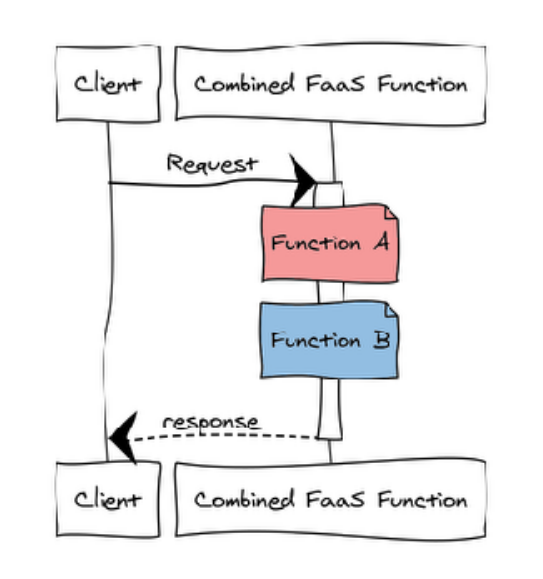
\includegraphics[width=80mm]{./thesis_images/manual_comp.png}
\label{fig:Manual compilation}
\end{figure}

\begin{lstlisting}
def funcA():
  doStuff()

def funcB():
  doStuff()

def main():
  funcA()
  funcB()
\end{lstlisting}

The above code block and Figure 4 explains how the control flow works in this
kind of compilation scheme. As is pretty obvious, with this method one cannot
scale individual functions independently and function can get really big. There
is no necessity to store intermediate data or serialize and deserialize data
between functions. But the problem is that this kind of violates the notion of
serverless since each application is not an atomic functional unit. If the
compute is complex, function might not even completely run because of the
hardbound limit to the running time set on most FaaS platforms. 

\paragraph{Direct function chaining}
\label{sec:org4213e1f}

\begin{figure}
\caption{Direct function chaining}
\centering
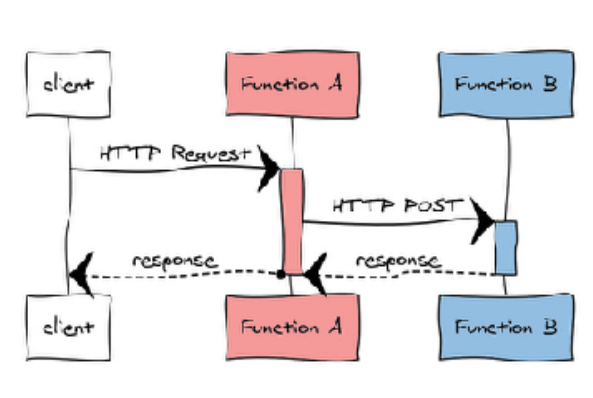
\includegraphics[width=90mm]{./thesis_images/func_chain.png}
\label{fig:Chaining}
\end{figure}

Like can be seen from Figure 5, here each task is a separate function. Each
function directly call the succeeding function in a chain. Meaning the code is
written so that the current knows the details of the next function, but not any
further. Even here like before, there is no need for any serialization
deserialization overhead since functions can directly send each other data. No
external components are used either. Although the problem arises when the data
load increases. The load on the network to transfer data via HTTP rises. Along
with that each function will have to wait for the next function. If a function
fails then the logic to retry/fallback etc. will have to be coded into each
function. The following pseudo code shows how the function design would be.


\begin{lstlisting}
def funcA():
  doStuff()
\end{lstlisting}


\begin{lstlisting}
def funcB():
  doStuff()
\end{lstlisting}

\paragraph{Composition via coordinator functions}
\label{sec:org10249e1}

In this method, a coordinator function will be used which manage the execution
of all the functions by calling them directly. The individual functions will be
unaware of each other. 

\begin{figure}
\caption{Coordination functions}
\centering
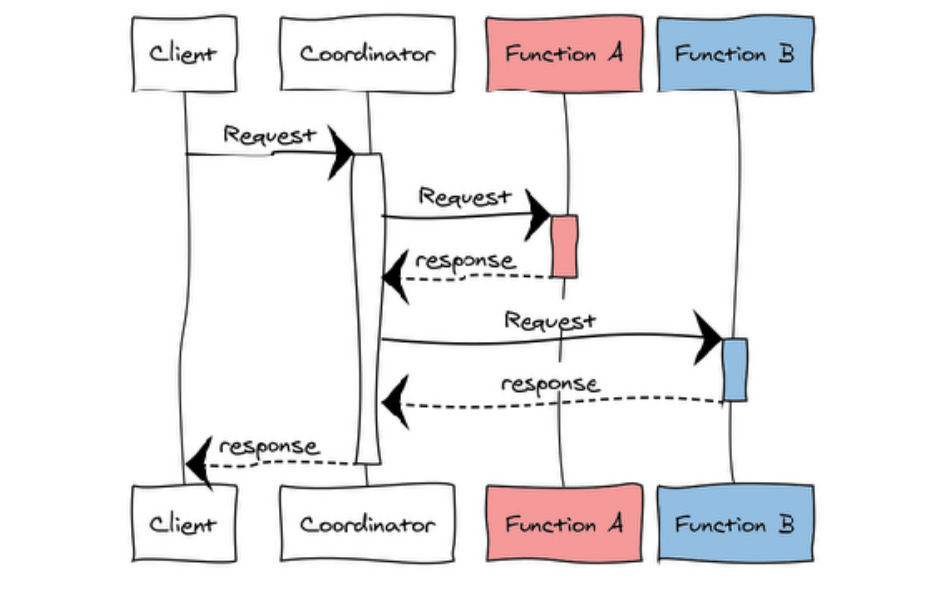
\includegraphics[width=150mm]{./thesis_images/coordination.png}
\label{fig:Coordination}
\end{figure}

The win over the previous method here is that, the house keeping code need not
be present in each individual task. Also it is very flexible in the sense that,
each function can be tested independently and then the user can properly write
the control flow in one place, that being the coordinator function. This comes
at a cost of adding an extra function which is the coordinator function. This
function will continue running the whole time, costing more and violating the
FaaS paradigm a bit. An example of this kind of coordination can be found here
CITE \{\href{https://www.researchgate.net/publication/331572138\_A\_framework\_and\_a\_performance\_assessment\_for\_serverless\_MapReduce\_on\_AWS\_Lambda}{PAPER}\}

\paragraph{Event driven composition}
\label{sec:org077f8d7}

\begin{figure}
\caption{Event driven function composition}
\centering
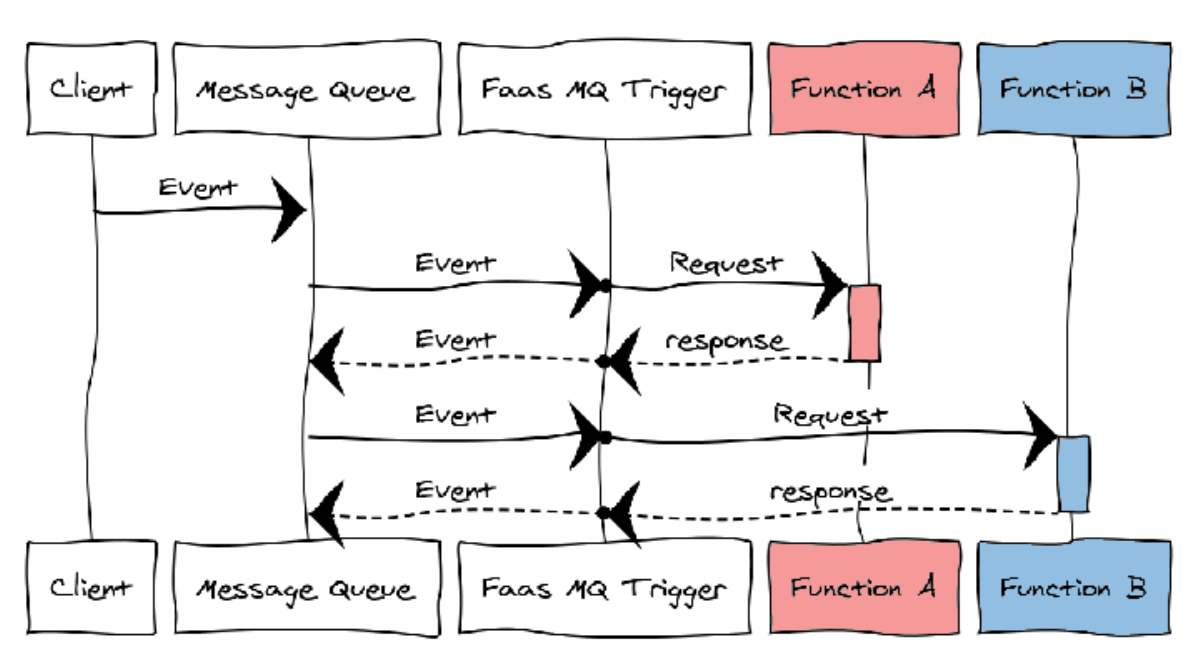
\includegraphics[width=150mm]{./thesis_images/event.png}
\label{fig:Event}
\end{figure}

This is a powerful design pattern that supports a lot more fault tolerance and
involves changing or extending the infrastructure of the FaaS platform. In this
method, one introduces message queues in the architecture as can be referred
from Figure 7. Functions emit events to these message queues. Alongside, all the
functions listen to the same queues. So on receiving certain events, they react
in the programmed ways. Contrary to all the previous methods, it is very
interesting to note that in this method, the stress is given to the data flow
instead of the control flow among functions. The intermediate data between the
functions has to be managed separately by using a storage.

This is a very commonly used and popular architecture. Message queues like Kafka
or MQTT brokers like rabitMQ offer a lot of functionalities and features like
fault tolerance, error handling, alerting, backup, etc. Functions can be
completely decoupled. This is a very good solution for big data and streaming
data applications.

The problem with this method is though the very heavy dependencies which are
very hard to manage. The fact that message queues are not inherently serverless
makes the platform less elastic and thereby billing and usage tracking can be
troublesome of the infrastructure manager. Alongside, message queues usually
only supports limited control flow structures. Probably just conditional and
on-error handles. It will be terribly complicated to do dynamic branching,
iterations, etc. Along with this, since functions are so tightly dependent on
the message queues, it will be slightly challenging to upgrade or version them. 

\paragraph{Workflows}
\label{sec:org60e0d5d}

Workflows are a very interesting architectures pattern where the system supports
the creation of a sort of flowchart of the functional interaction. Workflows are
a very widely used pattern these days in a lot of big data processing tools. 

An workflow is designed as a directed acyclic graph (DAG). This means that a new
runtime has to be introduced in the FaaS system to manage the execution of the
functions. When authoring a workflow, one should think how it could be divided
into tasks which can be executed independently. The workflow runtime would let
one to merge these tasks into a logical whole by combining them into a graph.

This definitely adds the overhead of writing a runtime for the FaaS platform,
providing an API to define the DAG to the runtime and then managing and
executing the workflow based on the DAGs. But once the platform is in place, it
provides numerous flexibility. One can get done dynamic branching, iteration,
etc. very easily on this platform along with individual upgrade of the
functions. The fact that no external infrastructure tool has to be managed to
work as a triggering mechanism maintains the elastic nature of the tool. The
only thing is that there has to be a storage unit to manage the state of the DAG
for the workflow framework. Similarly just the event driven composition, the
intermediate data store has to be handled separately.

Logically, this method resembles the coordinate function setup, just that
instead of a simple coordinator function, in this case we have a month more
powerful framework that is added permanently to the infrastructure. This can be
referred from Figure 8. 

\begin{figure}
\caption{Workflows}
\centering
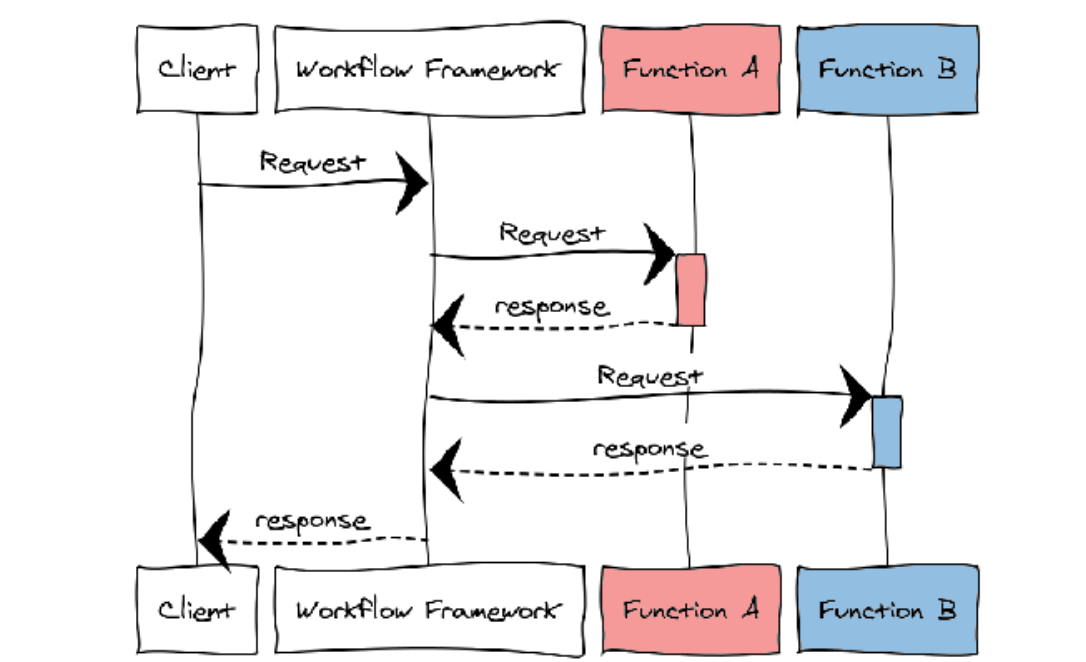
\includegraphics[width=150mm]{./thesis_images/workflow_2.png}
\label{fig:Workflows}
\end{figure}

The shape of the graph decides the overall logic of the workflow. A DAG can
include multiple branches and you can decide which of them to follow and which
to skip at the time of workflow execution. This creates a very resilient design,
because each task can be retried multiple times if an error occurs. To give the
reader clarity on what a DAG looks like, the Figure 9 from the Airflow's
operator might shed some light.

\begin{figure}
\caption{Branching example with DAGs}
\centering
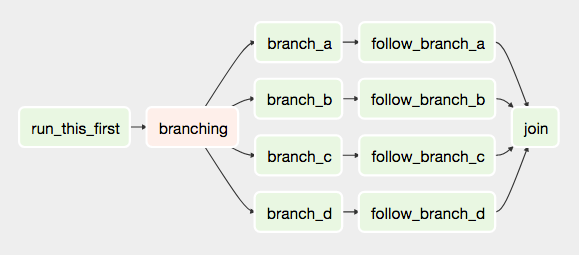
\includegraphics[width=80mm]{./thesis_images/workflow_1.png}
\label{fig:DAG}
\end{figure}







It is arguably clear that workflows offer the most flexible and application
independent solution as a 
\#+END\textsubscript{EXAMPLE}
\section{Implementation}
\label{sec:org46719c9}
\subsection{Tools}
\label{sec:orga41c270}
\subsubsection{Container Orchestration}
\label{sec:org8ff1f3c}
\subparagraph{Docker}
\label{sec:orga2e53d8}
\subparagraph{Kubernetes}
\label{sec:orge6fd97b}
\subsubsection{OpenFaaS}
\label{sec:org2a9315b}
\subsubsection{FaaS-flow}
\label{sec:orgf31d138}
\subsubsection{Pocket}
\label{sec:orgcdfda39}
\subsubsection{Prometheus}
\label{sec:org8324249}
\subsection{Architecture}
\label{sec:org42b222d}
\section{Evaluation}
\label{sec:org3c9e3f7}
\section{Future work}
\label{sec:org48cb3ef}
\section{Conclusion}
\label{sec:orgabaa607}


:UNNUMBERED: t
\end{document}
